\section{dfsch.h File Reference}
\label{dfsch_8h}\index{dfsch.h@{dfsch.h}}


This graph shows which files directly or indirectly include this file:\begin{figure}[H]
\begin{center}
\leavevmode
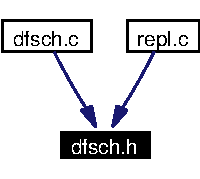
\includegraphics[width=65pt]{dfsch_8h__dep__incl}
\end{center}
\end{figure}
\subsection*{Defines}
\begin{CompactItemize}
\item 
\#define {\bf DFSCH\_\-CAR}\ 0\label{dfsch_8h_a0}

\item 
\#define {\bf DFSCH\_\-CDR}\ 0\label{dfsch_8h_a1}

\end{CompactItemize}
\subsection*{Typedefs}
\begin{CompactItemize}
\item 
typedef {\bf dfsch\_\-ctx\_\-t} {\bf dfsch\_\-ctx\_\-t}
\item 
typedef {\bf dfsch\_\-object\_\-t} {\bf dfsch\_\-object\_\-t}
\item 
typedef unsigned int {\bf dfsch\_\-c\-Xr\_\-t}
\item 
typedef {\bf dfsch\_\-object\_\-t} $\ast$($\ast$ {\bf dfsch\_\-primitive\_\-t} )({\bf dfsch\_\-object\_\-t} $\ast$)
\end{CompactItemize}
\subsection*{Functions}
\begin{CompactItemize}
\item 
int {\bf dfsch\_\-gc} ()
\item 
void {\bf dfsch\_\-object\_\-ref} ({\bf dfsch\_\-object\_\-t} $\ast$obj)
\item 
void {\bf dfsch\_\-object\_\-unref} ({\bf dfsch\_\-object\_\-t} $\ast$obj)
\item 
int {\bf dfsch\_\-eq\_\-p} ({\bf dfsch\_\-object\_\-t} $\ast$a, {\bf dfsch\_\-object\_\-t} $\ast$b)
\item 
int {\bf dfsch\_\-object\_\-null\_\-p} ({\bf dfsch\_\-object\_\-t} $\ast$obj)
\item 
int {\bf dfsch\_\-object\_\-pair\_\-p} ({\bf dfsch\_\-object\_\-t} $\ast$obj)
\item 
int {\bf dfsch\_\-object\_\-atom\_\-p} ({\bf dfsch\_\-object\_\-t} $\ast$obj)
\item 
int {\bf dfsch\_\-object\_\-symbol\_\-p} ({\bf dfsch\_\-object\_\-t} $\ast$obj)
\item 
int {\bf dfsch\_\-object\_\-number\_\-p} ({\bf dfsch\_\-object\_\-t} $\ast$obj)
\item 
int {\bf dfsch\_\-object\_\-string\_\-p} ({\bf dfsch\_\-object\_\-t} $\ast$obj)
\item 
int {\bf dfsch\_\-object\_\-primitive\_\-p} ({\bf dfsch\_\-object\_\-t} $\ast$obj)
\item 
int {\bf dfsch\_\-object\_\-closure\_\-p} ({\bf dfsch\_\-object\_\-t} $\ast$obj)
\item 
int {\bf dfsch\_\-object\_\-procedure\_\-p} ({\bf dfsch\_\-object\_\-t} $\ast$obj)
\item 
int {\bf dfsch\_\-object\_\-macro\_\-p} ({\bf dfsch\_\-object\_\-t} $\ast$obj)
\item 
int {\bf dfsch\_\-object\_\-exception\_\-p} ({\bf dfsch\_\-object\_\-t} $\ast$obj)
\item 
{\bf dfsch\_\-object\_\-t} $\ast$ {\bf dfsch\_\-obj\_\-read} (char $\ast$str)
\item 
char $\ast$ {\bf dfsch\_\-obj\_\-write} ({\bf dfsch\_\-object\_\-t} $\ast$obj, int max\_\-depth)
\item 
{\bf dfsch\_\-object\_\-t} $\ast$ {\bf dfsch\_\-nil} ()
\item 
{\bf dfsch\_\-object\_\-t} $\ast$ {\bf dfsch\_\-cons} ({\bf dfsch\_\-object\_\-t} $\ast$car, {\bf dfsch\_\-object\_\-t} $\ast$cdr)
\item 
{\bf dfsch\_\-object\_\-t} $\ast$ {\bf dfsch\_\-car} ({\bf dfsch\_\-object\_\-t} $\ast$pair)
\item 
{\bf dfsch\_\-object\_\-t} $\ast$ {\bf dfsch\_\-cdr} ({\bf dfsch\_\-object\_\-t} $\ast$pair)
\item 
{\bf dfsch\_\-object\_\-t} $\ast$ {\bf dfsch\_\-c\-Xr} ({\bf dfsch\_\-object\_\-t} $\ast$pair, {\bf dfsch\_\-c\-Xr\_\-t} x)
\item 
{\bf dfsch\_\-object\_\-t} $\ast$ {\bf dfsch\_\-set\_\-car} ({\bf dfsch\_\-object\_\-t} $\ast$pair, {\bf dfsch\_\-object\_\-t} $\ast$c)
\item 
{\bf dfsch\_\-object\_\-t} $\ast$ {\bf dfsch\_\-set\_\-cdr} ({\bf dfsch\_\-object\_\-t} $\ast$pair, {\bf dfsch\_\-object\_\-t} $\ast$c)
\item 
{\bf dfsch\_\-object\_\-t} $\ast$ {\bf dfsch\_\-assoc} ({\bf dfsch\_\-object\_\-t} $\ast$key, {\bf dfsch\_\-object\_\-t} $\ast$alist)
\item 
{\bf dfsch\_\-object\_\-t} $\ast$ {\bf dfsch\_\-make\_\-symbol} (char $\ast$symbol)
\item 
char $\ast$ {\bf dfsch\_\-symbol} ({\bf dfsch\_\-object\_\-t} $\ast$symbol)
\item 
{\bf dfsch\_\-object\_\-t} $\ast$ {\bf dfsch\_\-true} ()
\item 
{\bf dfsch\_\-object\_\-t} $\ast$ {\bf dfsch\_\-quote} ()
\item 
{\bf dfsch\_\-object\_\-t} $\ast$ {\bf dfsch\_\-make\_\-number} (double n)
\item 
float {\bf dfsch\_\-number} ({\bf dfsch\_\-object\_\-t} $\ast$n)
\item 
{\bf dfsch\_\-object\_\-t} $\ast$ {\bf dfsch\_\-lambda} ({\bf dfsch\_\-object\_\-t} $\ast$env, {\bf dfsch\_\-object\_\-t} $\ast$args, {\bf dfsch\_\-object\_\-t} $\ast$code)\label{dfsch_8h_a37}

\item 
{\bf dfsch\_\-object\_\-t} $\ast$ {\bf dfsch\_\-make\_\-primitive} ({\bf dfsch\_\-primitive\_\-t} prim)
\item 
{\bf dfsch\_\-object\_\-t} $\ast$ {\bf dfsch\_\-make\_\-macro} ({\bf dfsch\_\-object\_\-t} $\ast$proc)
\item 
{\bf dfsch\_\-object\_\-t} $\ast$ {\bf dfsch\_\-make\_\-exception} ({\bf dfsch\_\-object\_\-t} $\ast$type, {\bf dfsch\_\-object\_\-t} $\ast$data)
\item 
{\bf dfsch\_\-object\_\-t} $\ast$ {\bf dfsch\_\-lookup} ({\bf dfsch\_\-object\_\-t} $\ast$name, {\bf dfsch\_\-object\_\-t} $\ast$env)
\item 
{\bf dfsch\_\-object\_\-t} $\ast$ {\bf dfsch\_\-set} ({\bf dfsch\_\-object\_\-t} $\ast$name, {\bf dfsch\_\-object\_\-t} $\ast$value, {\bf dfsch\_\-object\_\-t} $\ast$env)
\item 
{\bf dfsch\_\-object\_\-t} $\ast$ {\bf dfsch\_\-define} ({\bf dfsch\_\-object\_\-t} $\ast$name, {\bf dfsch\_\-object\_\-t} $\ast$value, {\bf dfsch\_\-object\_\-t} $\ast$env)
\item 
{\bf dfsch\_\-object\_\-t} $\ast$ {\bf dfsch\_\-eval} ({\bf dfsch\_\-object\_\-t} $\ast$exp, {\bf dfsch\_\-object\_\-t} $\ast$env)
\item 
{\bf dfsch\_\-object\_\-t} $\ast$ {\bf dfsch\_\-apply} ({\bf dfsch\_\-object\_\-t} $\ast$proc, {\bf dfsch\_\-object\_\-t} $\ast$args)
\item 
{\bf dfsch\_\-ctx\_\-t} $\ast$ {\bf dfsch\_\-make\_\-context} ()
\item 
{\bf dfsch\_\-object\_\-t} $\ast$ {\bf dfsch\_\-ctx\_\-eval} ({\bf dfsch\_\-ctx\_\-t} $\ast$ctx, {\bf dfsch\_\-object\_\-t} $\ast$exp)
\item 
void {\bf dfsch\_\-destroy\_\-context} ({\bf dfsch\_\-ctx\_\-t} $\ast$ctx)
\item 
void {\bf dfsch\_\-ctx\_\-define} ({\bf dfsch\_\-ctx\_\-t} $\ast$ctx, char $\ast$name, {\bf dfsch\_\-object\_\-t} $\ast$obj)
\item 
{\bf dfsch\_\-object\_\-t} $\ast$ {\bf dfsch\_\-ctx\_\-environment} ({\bf dfsch\_\-ctx\_\-t} $\ast$ctx)\label{dfsch_8h_a50}

\end{CompactItemize}


\subsection{Detailed Description}
dfsch is quick and dirty implementation of someting that resembles scheme. This file contains interfacespecification.

Definition in file {\bf dfsch.h}.

\subsection{Typedef Documentation}
\index{dfsch.h@{dfsch.h}!dfsch_ctx_t@{dfsch\_\-ctx\_\-t}}
\index{dfsch_ctx_t@{dfsch\_\-ctx\_\-t}!dfsch.h@{dfsch.h}}
\subsubsection{\setlength{\rightskip}{0pt plus 5cm}typedef struct {\bf dfsch\_\-ctx\_\-t} {\bf dfsch\_\-ctx\_\-t}}\label{dfsch_8h_a2}


Interpreter context Definition at line 45 of file dfsch.h.\index{dfsch.h@{dfsch.h}!dfsch_cXr_t@{dfsch\_\-cXr\_\-t}}
\index{dfsch_cXr_t@{dfsch\_\-cXr\_\-t}!dfsch.h@{dfsch.h}}
\subsubsection{\setlength{\rightskip}{0pt plus 5cm}typedef unsigned int {\bf dfsch\_\-c\-Xr\_\-t}}\label{dfsch_8h_a4}


Meant for functions like caaddar, currently unused Definition at line 55 of file dfsch.h.\index{dfsch.h@{dfsch.h}!dfsch_object_t@{dfsch\_\-object\_\-t}}
\index{dfsch_object_t@{dfsch\_\-object\_\-t}!dfsch.h@{dfsch.h}}
\subsubsection{\setlength{\rightskip}{0pt plus 5cm}typedef struct {\bf dfsch\_\-object\_\-t} {\bf dfsch\_\-object\_\-t}}\label{dfsch_8h_a3}


C datatype for scheme objects Definition at line 50 of file dfsch.h.\index{dfsch.h@{dfsch.h}!dfsch_primitive_t@{dfsch\_\-primitive\_\-t}}
\index{dfsch_primitive_t@{dfsch\_\-primitive\_\-t}!dfsch.h@{dfsch.h}}
\subsubsection{\setlength{\rightskip}{0pt plus 5cm}typedef {\bf dfsch\_\-object\_\-t}$\ast$($\ast$ {\bf dfsch\_\-primitive\_\-t})({\bf dfsch\_\-object\_\-t} $\ast$)}\label{dfsch_8h_a5}


Native functions prototype Definition at line 60 of file dfsch.h.

\subsection{Function Documentation}
\index{dfsch.h@{dfsch.h}!dfsch_apply@{dfsch\_\-apply}}
\index{dfsch_apply@{dfsch\_\-apply}!dfsch.h@{dfsch.h}}
\subsubsection{\setlength{\rightskip}{0pt plus 5cm}{\bf dfsch\_\-object\_\-t}$\ast$ dfsch\_\-apply ({\bf dfsch\_\-object\_\-t} $\ast$ {\em proc}, {\bf dfsch\_\-object\_\-t} $\ast$ {\em args})}\label{dfsch_8h_a45}


Applyes procedure PROC to arguments ARGS. Obviously it doesn't work for macros. Definition at line 1336 of file dfsch.c.\index{dfsch.h@{dfsch.h}!dfsch_assoc@{dfsch\_\-assoc}}
\index{dfsch_assoc@{dfsch\_\-assoc}!dfsch.h@{dfsch.h}}
\subsubsection{\setlength{\rightskip}{0pt plus 5cm}{\bf dfsch\_\-object\_\-t}$\ast$ dfsch\_\-assoc ({\bf dfsch\_\-object\_\-t} $\ast$ {\em key}, {\bf dfsch\_\-object\_\-t} $\ast$ {\em alist})}\label{dfsch_8h_a30}


{\tt (assoc KEY ALIST)} Definition at line 542 of file dfsch.c.\index{dfsch.h@{dfsch.h}!dfsch_car@{dfsch\_\-car}}
\index{dfsch_car@{dfsch\_\-car}!dfsch.h@{dfsch.h}}
\subsubsection{\setlength{\rightskip}{0pt plus 5cm}{\bf dfsch\_\-object\_\-t}$\ast$ dfsch\_\-car ({\bf dfsch\_\-object\_\-t} $\ast$ {\em pair})}\label{dfsch_8h_a25}


{\tt (car PAIR)} Definition at line 498 of file dfsch.c.\index{dfsch.h@{dfsch.h}!dfsch_cdr@{dfsch\_\-cdr}}
\index{dfsch_cdr@{dfsch\_\-cdr}!dfsch.h@{dfsch.h}}
\subsubsection{\setlength{\rightskip}{0pt plus 5cm}{\bf dfsch\_\-object\_\-t}$\ast$ dfsch\_\-cdr ({\bf dfsch\_\-object\_\-t} $\ast$ {\em pair})}\label{dfsch_8h_a26}


{\tt (cdr PAIR)} Definition at line 505 of file dfsch.c.\index{dfsch.h@{dfsch.h}!dfsch_cons@{dfsch\_\-cons}}
\index{dfsch_cons@{dfsch\_\-cons}!dfsch.h@{dfsch.h}}
\subsubsection{\setlength{\rightskip}{0pt plus 5cm}{\bf dfsch\_\-object\_\-t}$\ast$ dfsch\_\-cons ({\bf dfsch\_\-object\_\-t} $\ast$ {\em car}, {\bf dfsch\_\-object\_\-t} $\ast$ {\em cdr})}\label{dfsch_8h_a24}


{\tt (cons CAR CDR)} Definition at line 487 of file dfsch.c.\index{dfsch.h@{dfsch.h}!dfsch_ctx_define@{dfsch\_\-ctx\_\-define}}
\index{dfsch_ctx_define@{dfsch\_\-ctx\_\-define}!dfsch.h@{dfsch.h}}
\subsubsection{\setlength{\rightskip}{0pt plus 5cm}void dfsch\_\-ctx\_\-define ({\bf dfsch\_\-ctx\_\-t} $\ast$ {\em ctx}, char $\ast$ {\em name}, {\bf dfsch\_\-object\_\-t} $\ast$ {\em obj})}\label{dfsch_8h_a49}


Defines new variable NAME with value OBJ in global environment of context CTX. Definition at line 1685 of file dfsch.c.\index{dfsch.h@{dfsch.h}!dfsch_ctx_eval@{dfsch\_\-ctx\_\-eval}}
\index{dfsch_ctx_eval@{dfsch\_\-ctx\_\-eval}!dfsch.h@{dfsch.h}}
\subsubsection{\setlength{\rightskip}{0pt plus 5cm}{\bf dfsch\_\-object\_\-t}$\ast$ dfsch\_\-ctx\_\-eval ({\bf dfsch\_\-ctx\_\-t} $\ast$ {\em ctx}, {\bf dfsch\_\-object\_\-t} $\ast$ {\em exp})}\label{dfsch_8h_a47}


Evaluates given expression EXP in global environment of given context CTX. Definition at line 1678 of file dfsch.c.\index{dfsch.h@{dfsch.h}!dfsch_cXr@{dfsch\_\-cXr}}
\index{dfsch_cXr@{dfsch\_\-cXr}!dfsch.h@{dfsch.h}}
\subsubsection{\setlength{\rightskip}{0pt plus 5cm}{\bf dfsch\_\-object\_\-t}$\ast$ dfsch\_\-c\-Xr ({\bf dfsch\_\-object\_\-t} $\ast$ {\em pair}, {\bf dfsch\_\-c\-Xr\_\-t} {\em x})}\label{dfsch_8h_a27}


Unimplemented \index{dfsch.h@{dfsch.h}!dfsch_define@{dfsch\_\-define}}
\index{dfsch_define@{dfsch\_\-define}!dfsch.h@{dfsch.h}}
\subsubsection{\setlength{\rightskip}{0pt plus 5cm}{\bf dfsch\_\-object\_\-t}$\ast$ dfsch\_\-define ({\bf dfsch\_\-object\_\-t} $\ast$ {\em name}, {\bf dfsch\_\-object\_\-t} $\ast$ {\em value}, {\bf dfsch\_\-object\_\-t} $\ast$ {\em env})}\label{dfsch_8h_a43}


Define variable name in environment env with initial value of value \index{dfsch.h@{dfsch.h}!dfsch_destroy_context@{dfsch\_\-destroy\_\-context}}
\index{dfsch_destroy_context@{dfsch\_\-destroy\_\-context}!dfsch.h@{dfsch.h}}
\subsubsection{\setlength{\rightskip}{0pt plus 5cm}void dfsch\_\-destroy\_\-context ({\bf dfsch\_\-ctx\_\-t} $\ast$ {\em ctx})}\label{dfsch_8h_a48}


Unregisters global environment of given context from list of non-deallocatable objects, runs garbage collector and dealocates memory taken by given context CTX. Definition at line 1681 of file dfsch.c.\index{dfsch.h@{dfsch.h}!dfsch_eq_p@{dfsch\_\-eq\_\-p}}
\index{dfsch_eq_p@{dfsch\_\-eq\_\-p}!dfsch.h@{dfsch.h}}
\subsubsection{\setlength{\rightskip}{0pt plus 5cm}int dfsch\_\-eq\_\-p ({\bf dfsch\_\-object\_\-t} $\ast$ {\em a}, {\bf dfsch\_\-object\_\-t} $\ast$ {\em b})}\label{dfsch_8h_a9}


Are A and B equal objects? Definition at line 403 of file dfsch.c.\index{dfsch.h@{dfsch.h}!dfsch_eval@{dfsch\_\-eval}}
\index{dfsch_eval@{dfsch\_\-eval}!dfsch.h@{dfsch.h}}
\subsubsection{\setlength{\rightskip}{0pt plus 5cm}{\bf dfsch\_\-object\_\-t}$\ast$ dfsch\_\-eval ({\bf dfsch\_\-object\_\-t} $\ast$ {\em exp}, {\bf dfsch\_\-object\_\-t} $\ast$ {\em env})}\label{dfsch_8h_a44}


Evaluates EXP in given binding environment ENV. Definition at line 1231 of file dfsch.c.\index{dfsch.h@{dfsch.h}!dfsch_gc@{dfsch\_\-gc}}
\index{dfsch_gc@{dfsch\_\-gc}!dfsch.h@{dfsch.h}}
\subsubsection{\setlength{\rightskip}{0pt plus 5cm}int dfsch\_\-gc ()}\label{dfsch_8h_a6}


Perform garbage collection Definition at line 258 of file dfsch.c.\index{dfsch.h@{dfsch.h}!dfsch_lookup@{dfsch\_\-lookup}}
\index{dfsch_lookup@{dfsch\_\-lookup}!dfsch.h@{dfsch.h}}
\subsubsection{\setlength{\rightskip}{0pt plus 5cm}{\bf dfsch\_\-object\_\-t}$\ast$ dfsch\_\-lookup ({\bf dfsch\_\-object\_\-t} $\ast$ {\em name}, {\bf dfsch\_\-object\_\-t} $\ast$ {\em env})}\label{dfsch_8h_a41}


Get value of variable name in environment env. \index{dfsch.h@{dfsch.h}!dfsch_make_context@{dfsch\_\-make\_\-context}}
\index{dfsch_make_context@{dfsch\_\-make\_\-context}!dfsch.h@{dfsch.h}}
\subsubsection{\setlength{\rightskip}{0pt plus 5cm}{\bf dfsch\_\-ctx\_\-t}$\ast$ dfsch\_\-make\_\-context ()}\label{dfsch_8h_a46}


Allocates new context and adds its top-level environment into list of objects tat sould not be dealocated by garbage collector. Definition at line 1611 of file dfsch.c.\index{dfsch.h@{dfsch.h}!dfsch_make_exception@{dfsch\_\-make\_\-exception}}
\index{dfsch_make_exception@{dfsch\_\-make\_\-exception}!dfsch.h@{dfsch.h}}
\subsubsection{\setlength{\rightskip}{0pt plus 5cm}{\bf dfsch\_\-object\_\-t}$\ast$ dfsch\_\-make\_\-exception ({\bf dfsch\_\-object\_\-t} $\ast$ {\em type}, {\bf dfsch\_\-object\_\-t} $\ast$ {\em data})}\label{dfsch_8h_a40}


Makes exception symbol of given TYPE and DATA. Definition at line 732 of file dfsch.c.\index{dfsch.h@{dfsch.h}!dfsch_make_macro@{dfsch\_\-make\_\-macro}}
\index{dfsch_make_macro@{dfsch\_\-make\_\-macro}!dfsch.h@{dfsch.h}}
\subsubsection{\setlength{\rightskip}{0pt plus 5cm}{\bf dfsch\_\-object\_\-t}$\ast$ dfsch\_\-make\_\-macro ({\bf dfsch\_\-object\_\-t} $\ast$ {\em proc})}\label{dfsch_8h_a39}


Wraps procedure for use as macro. \index{dfsch.h@{dfsch.h}!dfsch_make_number@{dfsch\_\-make\_\-number}}
\index{dfsch_make_number@{dfsch\_\-make\_\-number}!dfsch.h@{dfsch.h}}
\subsubsection{\setlength{\rightskip}{0pt plus 5cm}{\bf dfsch\_\-object\_\-t}$\ast$ dfsch\_\-make\_\-number (double {\em n})}\label{dfsch_8h_a35}


Makes number object from given floating-point number. Definition at line 569 of file dfsch.c.\index{dfsch.h@{dfsch.h}!dfsch_make_primitive@{dfsch\_\-make\_\-primitive}}
\index{dfsch_make_primitive@{dfsch\_\-make\_\-primitive}!dfsch.h@{dfsch.h}}
\subsubsection{\setlength{\rightskip}{0pt plus 5cm}{\bf dfsch\_\-object\_\-t}$\ast$ dfsch\_\-make\_\-primitive ({\bf dfsch\_\-primitive\_\-t} {\em prim})}\label{dfsch_8h_a38}


Makes primitive (native) procedure from pointer to implementing function. Definition at line 695 of file dfsch.c.\index{dfsch.h@{dfsch.h}!dfsch_make_symbol@{dfsch\_\-make\_\-symbol}}
\index{dfsch_make_symbol@{dfsch\_\-make\_\-symbol}!dfsch.h@{dfsch.h}}
\subsubsection{\setlength{\rightskip}{0pt plus 5cm}{\bf dfsch\_\-object\_\-t}$\ast$ dfsch\_\-make\_\-symbol (char $\ast$ {\em symbol})}\label{dfsch_8h_a31}


Makes symbol object from corresponding ASCIIZ string. Definition at line 641 of file dfsch.c.\index{dfsch.h@{dfsch.h}!dfsch_nil@{dfsch\_\-nil}}
\index{dfsch_nil@{dfsch\_\-nil}!dfsch.h@{dfsch.h}}
\subsubsection{\setlength{\rightskip}{0pt plus 5cm}{\bf dfsch\_\-object\_\-t}$\ast$ dfsch\_\-nil ()}\label{dfsch_8h_a23}


{\tt '()} \index{dfsch.h@{dfsch.h}!dfsch_number@{dfsch\_\-number}}
\index{dfsch_number@{dfsch\_\-number}!dfsch.h@{dfsch.h}}
\subsubsection{\setlength{\rightskip}{0pt plus 5cm}float dfsch\_\-number ({\bf dfsch\_\-object\_\-t} $\ast$ {\em n})}\label{dfsch_8h_a36}


Returns native representation of given number object; Definition at line 580 of file dfsch.c.\index{dfsch.h@{dfsch.h}!dfsch_obj_read@{dfsch\_\-obj\_\-read}}
\index{dfsch_obj_read@{dfsch\_\-obj\_\-read}!dfsch.h@{dfsch.h}}
\subsubsection{\setlength{\rightskip}{0pt plus 5cm}{\bf dfsch\_\-object\_\-t}$\ast$ dfsch\_\-obj\_\-read (char $\ast$ {\em str})}\label{dfsch_8h_a21}


Parse ASCIIZ string into object Definition at line 1008 of file dfsch.c.\index{dfsch.h@{dfsch.h}!dfsch_obj_write@{dfsch\_\-obj\_\-write}}
\index{dfsch_obj_write@{dfsch\_\-obj\_\-write}!dfsch.h@{dfsch.h}}
\subsubsection{\setlength{\rightskip}{0pt plus 5cm}char$\ast$ dfsch\_\-obj\_\-write ({\bf dfsch\_\-object\_\-t} $\ast$ {\em obj}, int {\em max\_\-depth})}\label{dfsch_8h_a22}


Convert object to ASCIIZ string Definition at line 1014 of file dfsch.c.\index{dfsch.h@{dfsch.h}!dfsch_object_atom_p@{dfsch\_\-object\_\-atom\_\-p}}
\index{dfsch_object_atom_p@{dfsch\_\-object\_\-atom\_\-p}!dfsch.h@{dfsch.h}}
\subsubsection{\setlength{\rightskip}{0pt plus 5cm}int dfsch\_\-object\_\-atom\_\-p ({\bf dfsch\_\-object\_\-t} $\ast$ {\em obj})}\label{dfsch_8h_a12}


Is A an atom? Definition at line 434 of file dfsch.c.\index{dfsch.h@{dfsch.h}!dfsch_object_closure_p@{dfsch\_\-object\_\-closure\_\-p}}
\index{dfsch_object_closure_p@{dfsch\_\-object\_\-closure\_\-p}!dfsch.h@{dfsch.h}}
\subsubsection{\setlength{\rightskip}{0pt plus 5cm}int dfsch\_\-object\_\-closure\_\-p ({\bf dfsch\_\-object\_\-t} $\ast$ {\em obj})}\label{dfsch_8h_a17}


Is A a lambda-closure?? Definition at line 461 of file dfsch.c.\index{dfsch.h@{dfsch.h}!dfsch_object_exception_p@{dfsch\_\-object\_\-exception\_\-p}}
\index{dfsch_object_exception_p@{dfsch\_\-object\_\-exception\_\-p}!dfsch.h@{dfsch.h}}
\subsubsection{\setlength{\rightskip}{0pt plus 5cm}int dfsch\_\-object\_\-exception\_\-p ({\bf dfsch\_\-object\_\-t} $\ast$ {\em obj})}\label{dfsch_8h_a20}


Is A an exception? Definition at line 477 of file dfsch.c.\index{dfsch.h@{dfsch.h}!dfsch_object_macro_p@{dfsch\_\-object\_\-macro\_\-p}}
\index{dfsch_object_macro_p@{dfsch\_\-object\_\-macro\_\-p}!dfsch.h@{dfsch.h}}
\subsubsection{\setlength{\rightskip}{0pt plus 5cm}int dfsch\_\-object\_\-macro\_\-p ({\bf dfsch\_\-object\_\-t} $\ast$ {\em obj})}\label{dfsch_8h_a19}


Is A an macro? Definition at line 471 of file dfsch.c.\index{dfsch.h@{dfsch.h}!dfsch_object_null_p@{dfsch\_\-object\_\-null\_\-p}}
\index{dfsch_object_null_p@{dfsch\_\-object\_\-null\_\-p}!dfsch.h@{dfsch.h}}
\subsubsection{\setlength{\rightskip}{0pt plus 5cm}int dfsch\_\-object\_\-null\_\-p ({\bf dfsch\_\-object\_\-t} $\ast$ {\em obj})}\label{dfsch_8h_a10}


Is A null? Definition at line 426 of file dfsch.c.\index{dfsch.h@{dfsch.h}!dfsch_object_number_p@{dfsch\_\-object\_\-number\_\-p}}
\index{dfsch_object_number_p@{dfsch\_\-object\_\-number\_\-p}!dfsch.h@{dfsch.h}}
\subsubsection{\setlength{\rightskip}{0pt plus 5cm}int dfsch\_\-object\_\-number\_\-p ({\bf dfsch\_\-object\_\-t} $\ast$ {\em obj})}\label{dfsch_8h_a14}


Is A a anumber? Definition at line 444 of file dfsch.c.\index{dfsch.h@{dfsch.h}!dfsch_object_pair_p@{dfsch\_\-object\_\-pair\_\-p}}
\index{dfsch_object_pair_p@{dfsch\_\-object\_\-pair\_\-p}!dfsch.h@{dfsch.h}}
\subsubsection{\setlength{\rightskip}{0pt plus 5cm}int dfsch\_\-object\_\-pair\_\-p ({\bf dfsch\_\-object\_\-t} $\ast$ {\em obj})}\label{dfsch_8h_a11}


Is A a pair? Definition at line 429 of file dfsch.c.\index{dfsch.h@{dfsch.h}!dfsch_object_primitive_p@{dfsch\_\-object\_\-primitive\_\-p}}
\index{dfsch_object_primitive_p@{dfsch\_\-object\_\-primitive\_\-p}!dfsch.h@{dfsch.h}}
\subsubsection{\setlength{\rightskip}{0pt plus 5cm}int dfsch\_\-object\_\-primitive\_\-p ({\bf dfsch\_\-object\_\-t} $\ast$ {\em obj})}\label{dfsch_8h_a16}


Is A a primitive (native) function? Definition at line 455 of file dfsch.c.\index{dfsch.h@{dfsch.h}!dfsch_object_procedure_p@{dfsch\_\-object\_\-procedure\_\-p}}
\index{dfsch_object_procedure_p@{dfsch\_\-object\_\-procedure\_\-p}!dfsch.h@{dfsch.h}}
\subsubsection{\setlength{\rightskip}{0pt plus 5cm}int dfsch\_\-object\_\-procedure\_\-p ({\bf dfsch\_\-object\_\-t} $\ast$ {\em obj})}\label{dfsch_8h_a18}


Is A an applicable procedure? Definition at line 466 of file dfsch.c.\index{dfsch.h@{dfsch.h}!dfsch_object_ref@{dfsch\_\-object\_\-ref}}
\index{dfsch_object_ref@{dfsch\_\-object\_\-ref}!dfsch.h@{dfsch.h}}
\subsubsection{\setlength{\rightskip}{0pt plus 5cm}void dfsch\_\-object\_\-ref ({\bf dfsch\_\-object\_\-t} $\ast$ {\em obj})}\label{dfsch_8h_a7}


Mark object as referenced from C code. \index{dfsch.h@{dfsch.h}!dfsch_object_string_p@{dfsch\_\-object\_\-string\_\-p}}
\index{dfsch_object_string_p@{dfsch\_\-object\_\-string\_\-p}!dfsch.h@{dfsch.h}}
\subsubsection{\setlength{\rightskip}{0pt plus 5cm}int dfsch\_\-object\_\-string\_\-p ({\bf dfsch\_\-object\_\-t} $\ast$ {\em obj})}\label{dfsch_8h_a15}


Is A a string? Definition at line 449 of file dfsch.c.\index{dfsch.h@{dfsch.h}!dfsch_object_symbol_p@{dfsch\_\-object\_\-symbol\_\-p}}
\index{dfsch_object_symbol_p@{dfsch\_\-object\_\-symbol\_\-p}!dfsch.h@{dfsch.h}}
\subsubsection{\setlength{\rightskip}{0pt plus 5cm}int dfsch\_\-object\_\-symbol\_\-p ({\bf dfsch\_\-object\_\-t} $\ast$ {\em obj})}\label{dfsch_8h_a13}


Is A a symbol? Definition at line 439 of file dfsch.c.\index{dfsch.h@{dfsch.h}!dfsch_object_unref@{dfsch\_\-object\_\-unref}}
\index{dfsch_object_unref@{dfsch\_\-object\_\-unref}!dfsch.h@{dfsch.h}}
\subsubsection{\setlength{\rightskip}{0pt plus 5cm}void dfsch\_\-object\_\-unref ({\bf dfsch\_\-object\_\-t} $\ast$ {\em obj})}\label{dfsch_8h_a8}


Unregister referenced object. \index{dfsch.h@{dfsch.h}!dfsch_quote@{dfsch\_\-quote}}
\index{dfsch_quote@{dfsch\_\-quote}!dfsch.h@{dfsch.h}}
\subsubsection{\setlength{\rightskip}{0pt plus 5cm}{\bf dfsch\_\-object\_\-t}$\ast$ dfsch\_\-quote ()}\label{dfsch_8h_a34}


Performance hack: returns symbol {\tt quote} witout need for looking it up every time. Definition at line 666 of file dfsch.c.\index{dfsch.h@{dfsch.h}!dfsch_set@{dfsch\_\-set}}
\index{dfsch_set@{dfsch\_\-set}!dfsch.h@{dfsch.h}}
\subsubsection{\setlength{\rightskip}{0pt plus 5cm}{\bf dfsch\_\-object\_\-t}$\ast$ dfsch\_\-set ({\bf dfsch\_\-object\_\-t} $\ast$ {\em name}, {\bf dfsch\_\-object\_\-t} $\ast$ {\em value}, {\bf dfsch\_\-object\_\-t} $\ast$ {\em env})}\label{dfsch_8h_a42}


Set value of variable name in environment env to value. \index{dfsch.h@{dfsch.h}!dfsch_set_car@{dfsch\_\-set\_\-car}}
\index{dfsch_set_car@{dfsch\_\-set\_\-car}!dfsch.h@{dfsch.h}}
\subsubsection{\setlength{\rightskip}{0pt plus 5cm}{\bf dfsch\_\-object\_\-t}$\ast$ dfsch\_\-set\_\-car ({\bf dfsch\_\-object\_\-t} $\ast$ {\em pair}, {\bf dfsch\_\-object\_\-t} $\ast$ {\em c})}\label{dfsch_8h_a28}


{\tt (set-car! PAIR C)} Definition at line 513 of file dfsch.c.\index{dfsch.h@{dfsch.h}!dfsch_set_cdr@{dfsch\_\-set\_\-cdr}}
\index{dfsch_set_cdr@{dfsch\_\-set\_\-cdr}!dfsch.h@{dfsch.h}}
\subsubsection{\setlength{\rightskip}{0pt plus 5cm}{\bf dfsch\_\-object\_\-t}$\ast$ dfsch\_\-set\_\-cdr ({\bf dfsch\_\-object\_\-t} $\ast$ {\em pair}, {\bf dfsch\_\-object\_\-t} $\ast$ {\em c})}\label{dfsch_8h_a29}


{\tt (set-cdr! PAIR C)} Definition at line 526 of file dfsch.c.\index{dfsch.h@{dfsch.h}!dfsch_symbol@{dfsch\_\-symbol}}
\index{dfsch_symbol@{dfsch\_\-symbol}!dfsch.h@{dfsch.h}}
\subsubsection{\setlength{\rightskip}{0pt plus 5cm}char$\ast$ dfsch\_\-symbol ({\bf dfsch\_\-object\_\-t} $\ast$ {\em symbol})}\label{dfsch_8h_a32}


Returns string representation of given symbol. Definition at line 651 of file dfsch.c.\index{dfsch.h@{dfsch.h}!dfsch_true@{dfsch\_\-true}}
\index{dfsch_true@{dfsch\_\-true}!dfsch.h@{dfsch.h}}
\subsubsection{\setlength{\rightskip}{0pt plus 5cm}{\bf dfsch\_\-object\_\-t}$\ast$ dfsch\_\-true ()}\label{dfsch_8h_a33}


Performance hack: returns symbol {\tt true} witout need for looking it up every time. Definition at line 657 of file dfsch.c.